\documentclass[licencjacka]{pracamgr}
\usepackage{polski}
\usepackage[utf8]{inputenc}
\usepackage[table]{xcolor}
\usepackage{array}
\usepackage{amssymb}
\usepackage{amsmath}
\usepackage{amsthm}
\usepackage[pdftex]{graphicx}
\usepackage{underscore}
\usepackage{hyperref}
\author{Tomasz Grabowski, Adam Markiewicz, Albert Rozmus, Krzysztof Rutkowski, Wiktor Zuba}
\nralbumu{305145, 334774, 248353, 319379, 320501}
\title{tytuł}
\tytulang{English title}
\kierunek{Informatyka}
\opiekun{dra Roberta Dąbrowskiego\\
Pion Zastępcy Kanclerza ds. Informatycznych}
\date{??? 2015}
\dziedzina{
11.0 Matematyka, Informatyka:\\
11.3 Informatyka\\
}
\klasyfikacja{
Information systems\\
Information systems applications\\
Decision support systems\\
Data analytics
}
%\TODO dodać litery/numery wierzchołków w klasyfikacji
\keywords{słowa kluczowe}
%\newtheorem{defi}{Definicja}[section]
\begin{document}
\maketitle
\begin{abstract}
Tu będzie abstract (skrót)
\end{abstract}
\tableofcontents
\chapter*{Wstęp}

Celem projektu było stworzenie serwisu internetowego zintegrowanego z systemem USOS 
wspierającego studentów w procesie świadomego doboru przedmiotów i konstruowania spójnego planu zajęć oraz
umożliwiającego studentom lepsze planowanie ścieżki studiów i kariery zawodowej
poprzez proponowanie przedmiotów, które mogą pasować do upodobań konkretnego studenta ocenionych na podstawie dotychczas wybieranych przedmiotów i otrzymywanych z nich ocen.
Dodatkowym wymaganiem projektu było oferowanie usług przewidywania dla konkretnych studentów ocen z przedmiotów, których jescze nie ukończyli lub nawet nie podjęli,
oraz przewidywania dla uniwersytetu ilości studentów którzy zapiszą się na konkretny przedmiot.
\addcontentsline{toc}{chapter}{Wprowadzenie}
 \chapter{Architektura}
 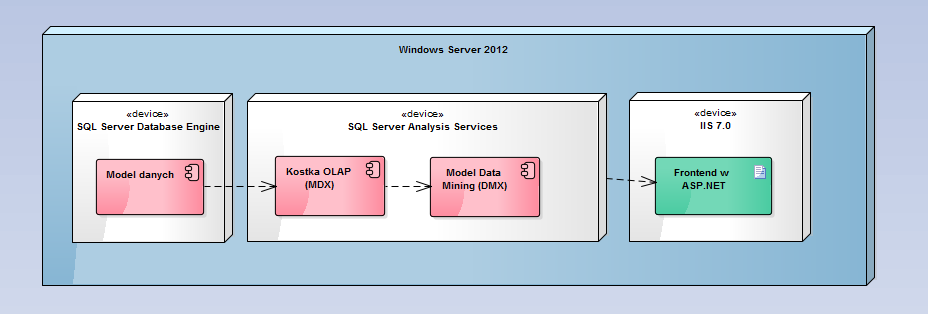
\includegraphics[scale=0.6]{Architektura.png}\newline
\begin{thebibliography}{99}
\addcontentsline{toc}{chapter}{Bibliografia}
\bibitem[abc]{ABC} Książka 1
\bibitem[def]{DEF} Link 2
\end{thebibliography}
\end{document}